

%% Chapter 1
%
\chapter{BREAK: Expansion Sets of Words} % Chapter title
%
\label{ch:expand} % For referencing the chapter elsewhere, use \autoref{ch:name} 
%
A typical text-based search engine system tokenizes queries and documents into words and uses heuristics to return a ranked list of relevant documents to the query.
This analogy can be extended towards string-related operations, where instead of dividing a sentence into words, one could divide a string into small chunks.

The \textit{k-grams} splitting technique illustrates the trivial chunking.
The word \textit{pizza} is split with $k = 2$ as: $\left\lbrace \langle \textit{s} \rangle \textit{p, pi, iz, zz, za, a} \langle / \textit{s} \rangle \right\rbrace$. 
Here, $\langle \textit{s} \rangle$ is the start token and $\langle / \textit{s} \rangle$ is the stop token.
For the sake of the simplicity, we have ignored terminal tokens in the k-gram splits.
Hence, the split set looks like: $\left\lbrace \textit{p, pi, iz, zz, za, a} \right\rbrace$. 
We would label this approach as BREAK-0 because it splits the words into smaller $k$-grams without any sequential information.

\section{BREAK-1: Sequencing from 1 End}
We argue that BREAK-0 could lead to an extremely generalized matching of tokens since an expansion set could be visualized a bag-of-words method. 
Thus, we propose a positional k-gram splitting technique, BREAK-1 which introduces position number in the splits to incorporate the notion of the sequence of the tokens in the word. 
For example, the word \textit{pizza} could be position-wise split with $k = 2$ as: $\left\lbrace \textit{1p, 2pi, 3iz, 4zz, 5za, 6a} \right\rbrace$. 
Thus, the member \textit{4zz} simply means that it is the fourth member of the set.
The motivation behind this tweak is that it gives us a rough amount of sequential-insight for spelling splits when they are used in probabilistic retrieval ranking functions.

\section{BREAK-2: Sequencing from 2 Ends}
The main disadvantage of the BREAK-1 is that some misspellings can easily disturb the order of the set which leads to low similarity.
For example, if the misspelling (query) is \textit{ppizza}, the split set would be $\left\lbrace \textit{1p, 2pp, 3pi, 4iz, 5zz, 6za, 7a} \right\rbrace$.
The order of the members after \textit{2pp} is misplaced, thus this would lead to low similarity with the correct spelling (document) $\left\lbrace \textit{1p, 2pi, 3iz, 4zz, 5za, 6a} \right\rbrace$. 
Only $\left\lbrace \textit{1p} \right\rbrace$ is common between correct and incorrect spell-splits.
Hence, we propose BREAK-2, a split algorithm which is robust against such displacements.

We attach position number to the left if the numbering begins from the start, and to the right if the numbering begins from the end.
Then the smallest position number would be selected between the two position numbers.
If the position numbers are equal, then we select the left position number as a convention.
Figure \ref{algo} gives an exemplification of this algorithm illustrated with splits of \textit{pizza} and \textit{hearts}.

\begin{figure}[h]
	\centering
	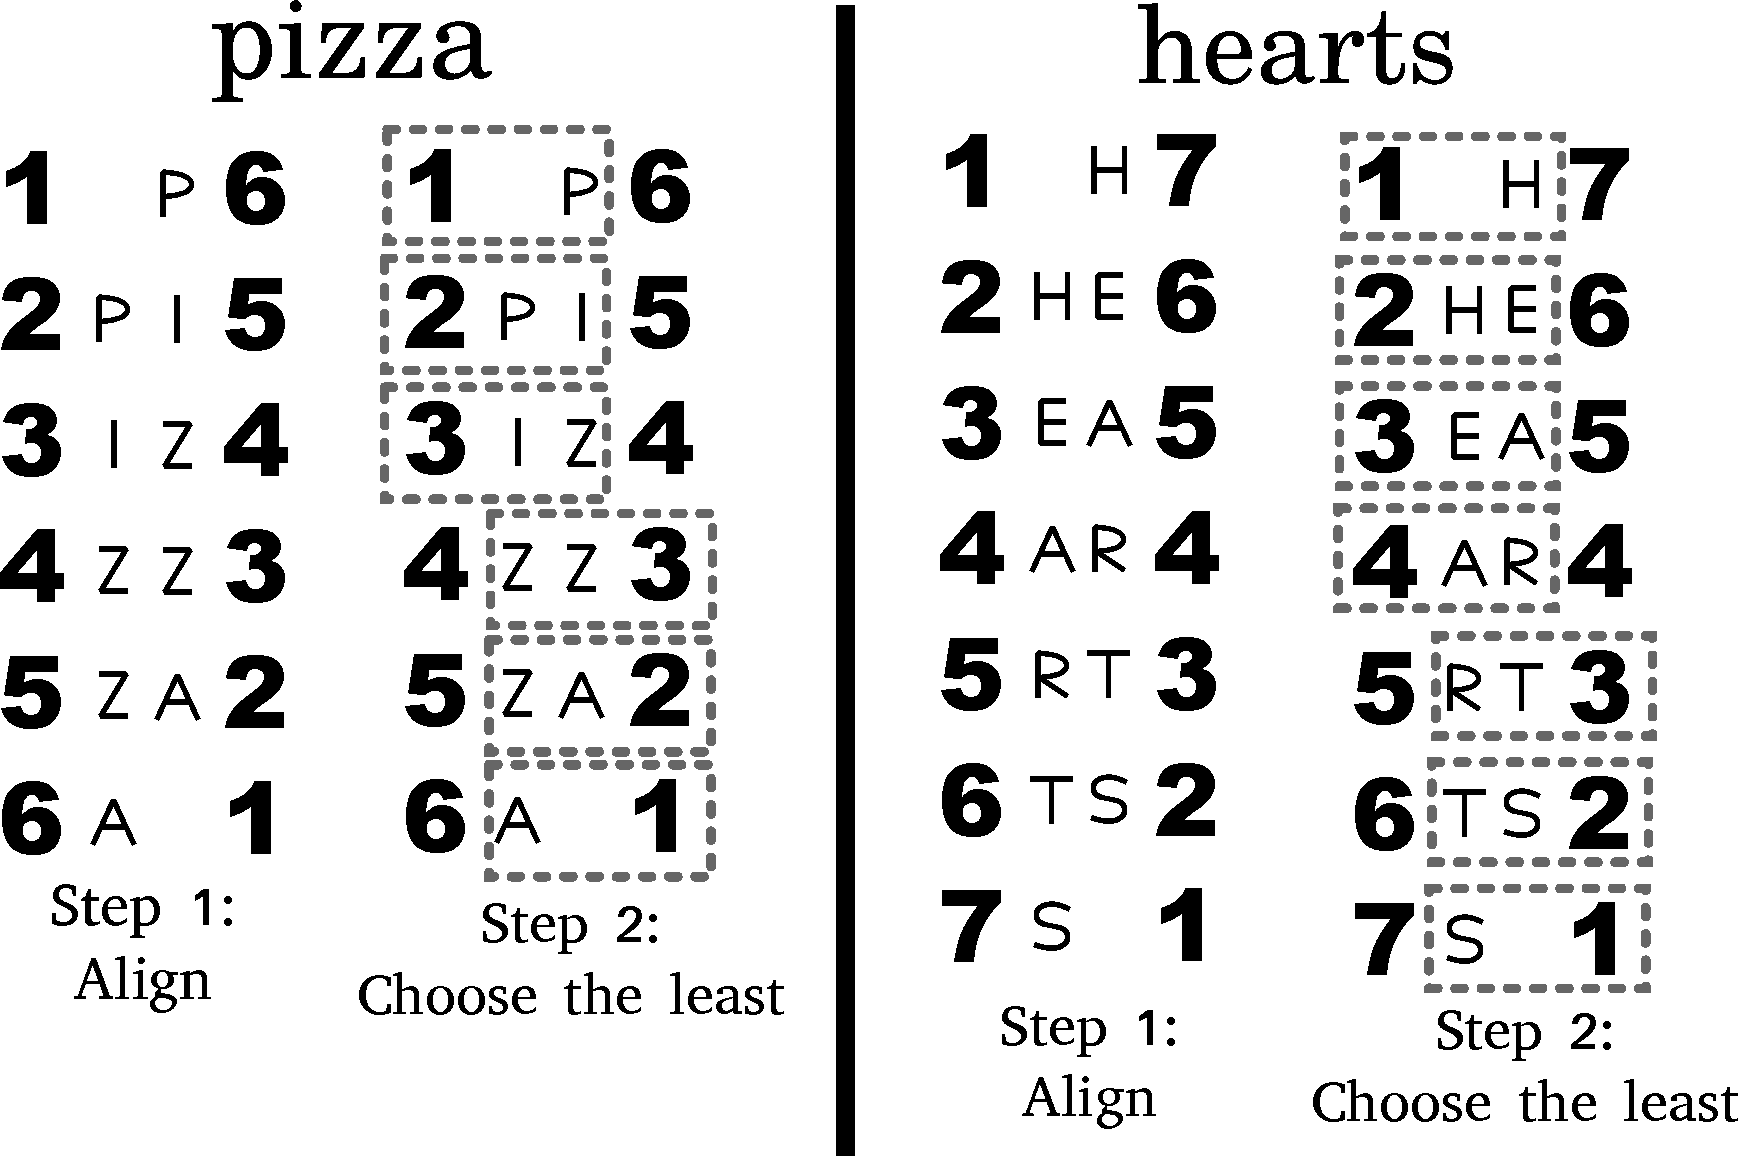
\includegraphics[width=\textwidth]{gfx/alg.pdf}
	\caption{The process of BREAK-2. On the left, algorithm slices pizza into pieces. The output set would be $\left\lbrace \textit{1p, 2pi, 3iz, zz3, za2, a1} \right\rbrace$. On the right, algorithm breaks hearts into pieces. The output set would be $\left\lbrace \textit{1h, 2he, 3ea, 4ar, rt3, ts2, s1} \right\rbrace$. }
	\label{algo}
\end{figure}
If the misspelling is \textit{ppizza}, the double-end split set would be $\left\lbrace \textit{1p, 2pp, 3pi, 4iz, zz3, za2, a1} \right\rbrace$. 
Thus it gives higher similarity with the correct spelling (document) as compared to positional split, as the set members $\left\lbrace \textit{1p, zz3, za2, a1} \right\rbrace$ would be matched.

\section{BREAK-Off: Sequencing with Offsets} 
We propose another variant, BREAK-\textit{X}-Off, which introduces offsets in the split-sets. 
(Here \textit{X} stands for the BREAK variant number used).
Let the BREAK-1 of pizza be $$S_0 = \lbrace \textit{1p, 2pi, 3iz, 4zz, 5za, 6a} \rbrace$$ which has no offsets.
An offset of $1$ would mean the counts would be displaced by 1, which is, $S_1 = \left\lbrace \textit{2p, 3pi, 4iz, 5zz, 6za, 7a} \right\rbrace$.
An offset of -1 would mean the counts would be displaced by -1, which is, $S_{-1} = \left\lbrace \textit{0p, 1pi, 2iz, 3zz, 4za, 5a} \right\rbrace$.
Now the complete split-up would be, thus , $S = S_{-1} \cup S_0 \cup S_1$. 
Similarly, offsets can be applied to the BREAK-2 splits too.

The motivation behind BREAK-\textit{X}-Off is that inclusion of offsets would be robust against the incorrect query provided.
For example, a spelling typographical error could have been caused by the insertion or deletion of the letter. 
Such insertions and deletions would displace the position sequences for the chunks. 
So the key here is to already index these possible errors, like for insertion, it would have an offset of 1 and for deletion, it would have an offset of -1.

For example, the split set for \textit{pizza} which was originally $$\left\lbrace \textit{1p, 2pi, 3iz, 4zz, 5za, 6a} \right\rbrace$$ after adding positional offset of $1$ looks like: $$\left\lbrace \textit{2p, 3pi, 4iz, 5zz, 6za, 7a} \right\rbrace$$
Offset with double-ended split-set now looks like $$\left\lbrace \textit{2p, 3pi, 4iz, zz4, za3, a2} \right\rbrace$$
For deletion errors, positional offset of -1 is included.
For example, the split set for \textit{pizza} after adding positional offset of -1 looks like: $$\left\lbrace \textit{0p, 1pi, 2iz, 3zz, 4za, 5a} \right\rbrace$$
Offset with double-ended split-set now looks like $$\left\lbrace \textit{0p, 1pi, 2iz, zz2, za1, a0} \right\rbrace$$
The complete split-set would include offsets of -1, 0 and 1. 
Thus, complete split-set of \textit{pizza} now looks like,
\begin{equation*}
	\begin{aligned}
		&\lbrace \textit{0p, 1pi, 2iz, zz2, za1, a0, 1p, 2pi, 3iz,} \\ 
		&\quad \textit{zz3, za2, a1, 2p, 3pi, 4iz, zz4, za3, a2} \rbrace
	\end{aligned}
\end{equation*}
However, set members $\left\lbrace \textit{0p, a0, 2p, a2} \right\rbrace$ are unlikely to happen as the numbering always starts from 1.
Hence we can ignore these members.
The final set is now,
\begin{equation*}
	\begin{aligned}
		C &= \lbrace \textit{1pi, 2iz, zz2, za1, 1p, 2pi, 3iz,} \\ 
		&\quad \textit{zz3, za2, a1, 3pi, 4iz, zz4, za3} \rbrace
	\end{aligned}
\end{equation*}
where $C$ is the correct split-set. 

Let the misspelling (query) be entered as \textit{piza}. The $I$, incorrect split-set by this method would be:
\begin{equation*}
	\begin{aligned}
		I &= \lbrace \textit{1pi, 2iz, za1, 1p, 2pi,} \\ 
		&\quad \textit{3iz, za2, a1, 3pi, 4iz, za3} \rbrace
	\end{aligned}
\end{equation*}
Then the match $C \cap I$ is,
\begin{equation*}
	\begin{aligned}
		C \cap I &= \lbrace \textit{1pi, 2iz, za1, 1p, 2pi,} \\ 
		&\quad \textit{3iz, za2, a1, 3pi, 4iz, za3} \rbrace
	\end{aligned}
\end{equation*}
Thus this method received more number of term matches, $ | C  \cap I | $ than any other methods. Similarly this method can be visualized for other types of spelling errors like insertion of letters. 


\section{BREAK-n: Sequential Splits for Longer Terms}

The main drawback of BREAK-2 algorithm is that the double-ended counts would be inefficient for the longer words. 
With elongation, the advantage of having two extremities would fade away, causing a similar drawback like BREAK-1.
This is undesirable for the non-natural language processing tasks like genome sequence analysis where a typical genetic sequence can be of thousands of base-pairs long.
In this section, we tackle this problem by proposing BREAK-n algorithm, which would generalize BREAK-2 and workaround for longer words.
\subsection{Anchoring}
Here, we introduce the notion of the anchor points.
Notice that in BREAK-2 algorithm, we numbered the terms from two extremities.
Now, instead of 2 extremities here, we number the terms relative to the $n$ extremities or \textit{anchor points}.
For a sequence with a length $l$, divided into $k$-grams and $n$ anchor points, the position of the $i^{th}$ anchor point ($pos_i$) is given by,
\begin{align}
	\label{anchor}
	pos_i = 1 + \frac{(i - 1)(l + k - 2)}{n - 1}
\end{align}
Each anchor point $i$ would have a corresponding vector $t_{e,i}$ having $j$ entries.
Every $t_{e, ij}$ entry will have information about the distance between $i^{th}$ anchor point and their position $j$.
Or simply,
\begin{align}
	\label{relative}
	t_{e, ij} = |pos_i - j|
\end{align}
Here $e$ stands for entity which can be either a document $d$, or query $q$.
We have illustrated a basic example in figure \ref{breakn} to exemplify this process.
\begin{figure}[h]
	\centering
	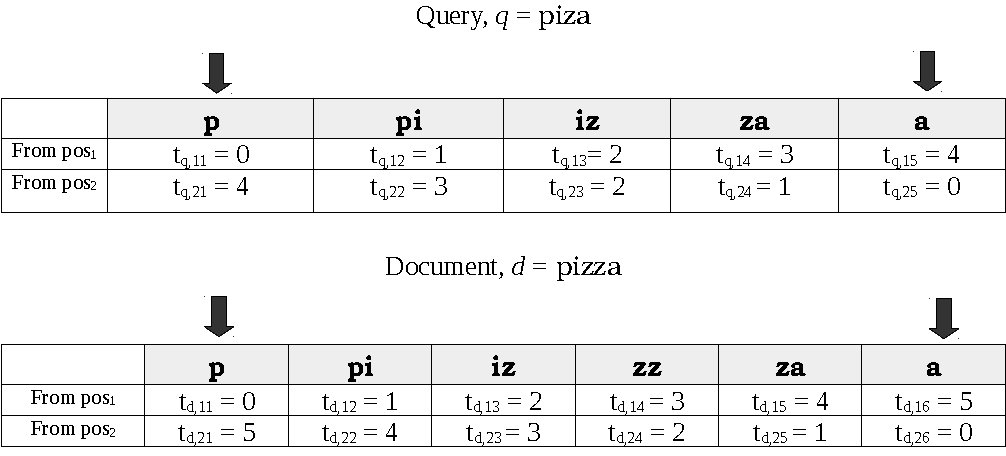
\includegraphics[width=\textwidth]{gfx/break-n.pdf}
	\caption{In this example, the words \textit{piza} and \textit{pizza} are given as $q$ and $d$ respectively, split into 2-grams. If we chose 2 anchor points, the position according to equation \ref{anchor} would be at the first and the last (which are shown in arrows). Now we fill every $t_{e, ij}$ entry by calculating relative distance given in equation \ref{relative}.}
	\label{breakn}
\end{figure}

\subsection{Redefining Intersection}
Comparing the analogy from BREAK-2, we impose conditional intersection here.
A term $t_q$ in query and $t_d$ in document is said to be \textit{completely intersected} if any of their relative positions from anchor points are same.
To achieve this, we would investigate their column vectors at the matched positions.

Let the matching position for $t_q$ and $t_d$ be $p_1$ and $p_2$, respectively.
We would extract $p_1$ and $p_2$ column vectors and check their corresponding indices for every anchor point.
Afterwards, we extract $p_1$ and $p_2$ column vectors, $t_{q, :p_1}$ and $t_{d, :p_2}$ respectively.
Then we would see if any of their corresponding indices are same.
If this happens, we say that they are \textit{completely intersected}.
In other words, any of the cells in the absolute difference between $t_{q, :p_1}$ and $t_{d, :p_2}$ should be 0.
Mathematically,
\begin{align}
	\label{intersect}
	\prod_{i = 1}^{n} |t_{q, ip_1} - t_{d, ip_2}| = 0
\end{align}
where $n$ is the length of the column vector (number of the anchor points).
If the resulting product around 0 is achieved, we would say that the term intersects completely between query and document.

Continuing the example from figure \ref{breakn}, let's assess the term \textit{za} which is common between $t_q$ ($p_1 = 3$) and $t_d$ ($p_2 = 4$). 
The $t_q$ column vector at $p_1 = 3$ is $t_{q, :3} = [3 \; 1]^T$ and for $t_d$ at $p_2 = 4$ is $t_{d, :4} = [4 \; 1]^T$.
Applying the equation \ref{intersect}, we get $\left(|3 - 4|\right) \left(|1 - 1|\right) = 0$, which means the term \textit{za} is completely intersected.
Analytically, this makes sense because position of \textit{za} from last is same in the two entities, and hence it should be completely intersected.
Although here we have shown the example of BREAK-n for a small word with two anchor points but BREAK-n can be logically extended to longer words with more anchor points.

\section{Combining BREAK with Ranking Functions}
Before indexing the documents, the dataset must be split according to the desired BREAK variant.
For the usage of BREAK-n, note that one can store the positional vectors while indexing the corresponding term, or generate the vector directly during evaluation.
This choice highly depends on the time-space tradeoff.
However, in our experiments we have stored the vectors during indexing, prioritizing faster evaluation. 

We have also combined length penalization heuristics (TAKE) with the probabilistic retrieval functions. 
The role of these heuristics is to reward the documents which are in closer to the length of the query.
This can be useful in the spell correction and cognate detection experiments as misspellings do not much absolute length difference with the correct spelled ones.
These length penalization heuristics can replace the conventional length normalization heuristics which are used in BM25 and Dirichlet.
In addition, we have also introduced graphical error models (MAKE) to analyze the confusion matrix generated during experimentation. 
The motivation behind this creation of graphical error model is to aid the identification and suggestion of solutions to the most probabilistic errors.